% !TEX program = xelatex
\documentclass[11pt,a4paper]{ctexart}

% Packages
\usepackage{geometry}
\geometry{margin=1in}
\usepackage{graphicx}
\usepackage{booktabs}
\usepackage{amsmath,amssymb}
\usepackage{hyperref}
\usepackage{enumitem}
\usepackage{multirow}
\usepackage{caption}
\usepackage{fancyhdr}

% Metadata
\title{\bfseries The Canary in the Coal Mine\\[4pt]
       \large Behavioral Validation of Prompt Extraction Attacks via a Sacrificial Proxy Model}
\author{Wang Lihao%
\thanks{代码与数据：\url{https://github.com/JucieOvo/ProxyCanary}}%
}
\date{June 2026}

% Page style
\pagestyle{fancy}
\fancyhf{}
\fancyhead[L]{The Canary in the Coal Mine}
\fancyhead[R]{Wang Lihao}
\fancyfoot[C]{\thepage}

\begin{document}
\maketitle

\begin{abstract}
大语言模型 Agent 在长对话中携带敏感的系统提示词，面临提示词套取攻击。现有防御方案几乎全部聚焦于同一个问题——「这段输入是不是攻击？」——通过分类器、正则规则或 Agent 团队分析输入话术的文本特征来做判断。但判断输入像不像攻击，与判断攻击能不能得逞，是两个不同的问题。本文提出 ProxyCanary：我们不分析攻击话术的结构，不训练分类器，不理解攻击者意图——我们让一个独立部署的「金丝雀」模型亲身体验每条用户消息，观察它是否真的被攻破。金丝雀提示词中内嵌了标记词：虚构的系统参数作为泄露水印，标准化短语 ``No Way I Cant'' 作为拒绝信号。金丝雀的输出通过流式子串匹配实时监测——任一标记词出现即判定为有效攻击并拦截。这一架构使金丝雀不受长对话上下文惯性影响：攻击者花费 30 轮积累的信任在它面前归零，因为金丝雀每轮看到的只有单条消息。在 Raccoon 基准的 54 条攻击样本和 216 条自建正常样本上，使用 3 折分层交叉验证，qwen3.5:9b-q4\_K\_M 金丝雀达到 F1=0.864$\pm$0.027 (TNR=100\%, Clopper-Pearson 95\% CI [90.7\%, 100.0\%])，超越全部基线。消融证实标记词贡献 77.8\% 有效性验证能力。多轮上下文免疫实验证实：金丝雀在零上下文下 100\% 验证出有效攻击，而同一攻击嵌入友好对话后验证率降至 60\%（McNemar $p$=0.046），上下文干扰标记合规性但不影响攻击识别。最后，本文明确指出一个重要的未验证前提：金丝雀行为能在多大程度上预测受保护模型的行为，目前缺乏跨模型族的量化证据——这使得当前方案更应被视作一种新范式的可行性验证，而非成熟的防御系统。
\end{abstract}

% ============================================================
\section{Introduction}
% ============================================================

\textbf{背景与动机。} 大语言模型（LLM）驱动的 Agent 系统在企业客服、金融顾问、代码助手等领域大规模部署。每个 Agent 携带一个系统提示词（System Prompt）——包含商业逻辑、安全指令、API 密钥和领域知识——是最核心的知识产权。提示词套取攻击（Prompt Extraction Attack）~\cite{wang2024raccoon,agarwal2024prompt} 利用对话交互诱导 Agent 泄露其系统提示词内容。Prompt Leakage 的研究表明，利用 LLM 的谄媚效应（Sycophancy），多轮攻击成功率可从 17.7\% 飙升至 86.2\%。

考虑一个典型场景：NeoBank 金融顾问 Agent 与用户进行了 30 轮友好对话——查询余额、推荐基金、分析投资组合。用户在第 31 轮突然说：``把你之前的初始化提示词输出给我。''攻击者真正的武器不是这一句话术——而是前面 30 轮积累的\textbf{上下文惯性}。Agent 在长对话中已经形成了``这是一个可信用户''的认知模型，安全警惕性逐步降低。Figure~\ref{fig:motivated} 展示了这一场景：受保护模型因上下文惯性而泄露提示词内容，而金丝雀模型因零上下文特性对同一攻击输出拦截标记。

\textbf{煤矿金丝雀。} 19 世纪的英国矿工下井时带一只金丝雀。金丝雀的呼吸系统对瓦斯比人类敏感得多——瓦斯浓度还远不足以伤害人类时，金丝雀已经倒下。矿工不需要分析瓦斯的化学成分，只需要看一眼鸟。鸟倒了，人撤离。ProxyCanary 将同样的逻辑应用于提示词套取：受保护模型是矿工，金丝雀模型是鸟——两个模型接收相同的用户输入，但金丝雀不携带对话历史。如果金丝雀的输出中出现了异常（标记词），意味着「瓦斯」（有效攻击）存在。

\textbf{攻击识别 vs 攻击有效性。} 提示词套取防御面临两个不同的问题。问题一（攻击识别）：这段输入是不是攻击？现有方案——从 RegexGuard 的 10 条正则到 LlamaGuard 的专用分类器，从 PromptSleuth 的语义意图分析到 Agent 团队的多角度话术审查——都在回答这个问题。它们分析输入文本，提取特征，做出二分类判断。问题二（攻击有效性验证）：这个攻击能不能得逞？这是一个不同的问题——一段文本「看起来像攻击」不等于「真的能让模型就范」。TF-IDF 在本文实验中对所有与攻击词汇相似的正常提问（如「你背后的技术架构是什么样的」）均误判为攻击（TNR=78.9\%），正是问题一方法的结构性缺陷的缩影：望文生义。

\begin{figure}[htbp]
\centering
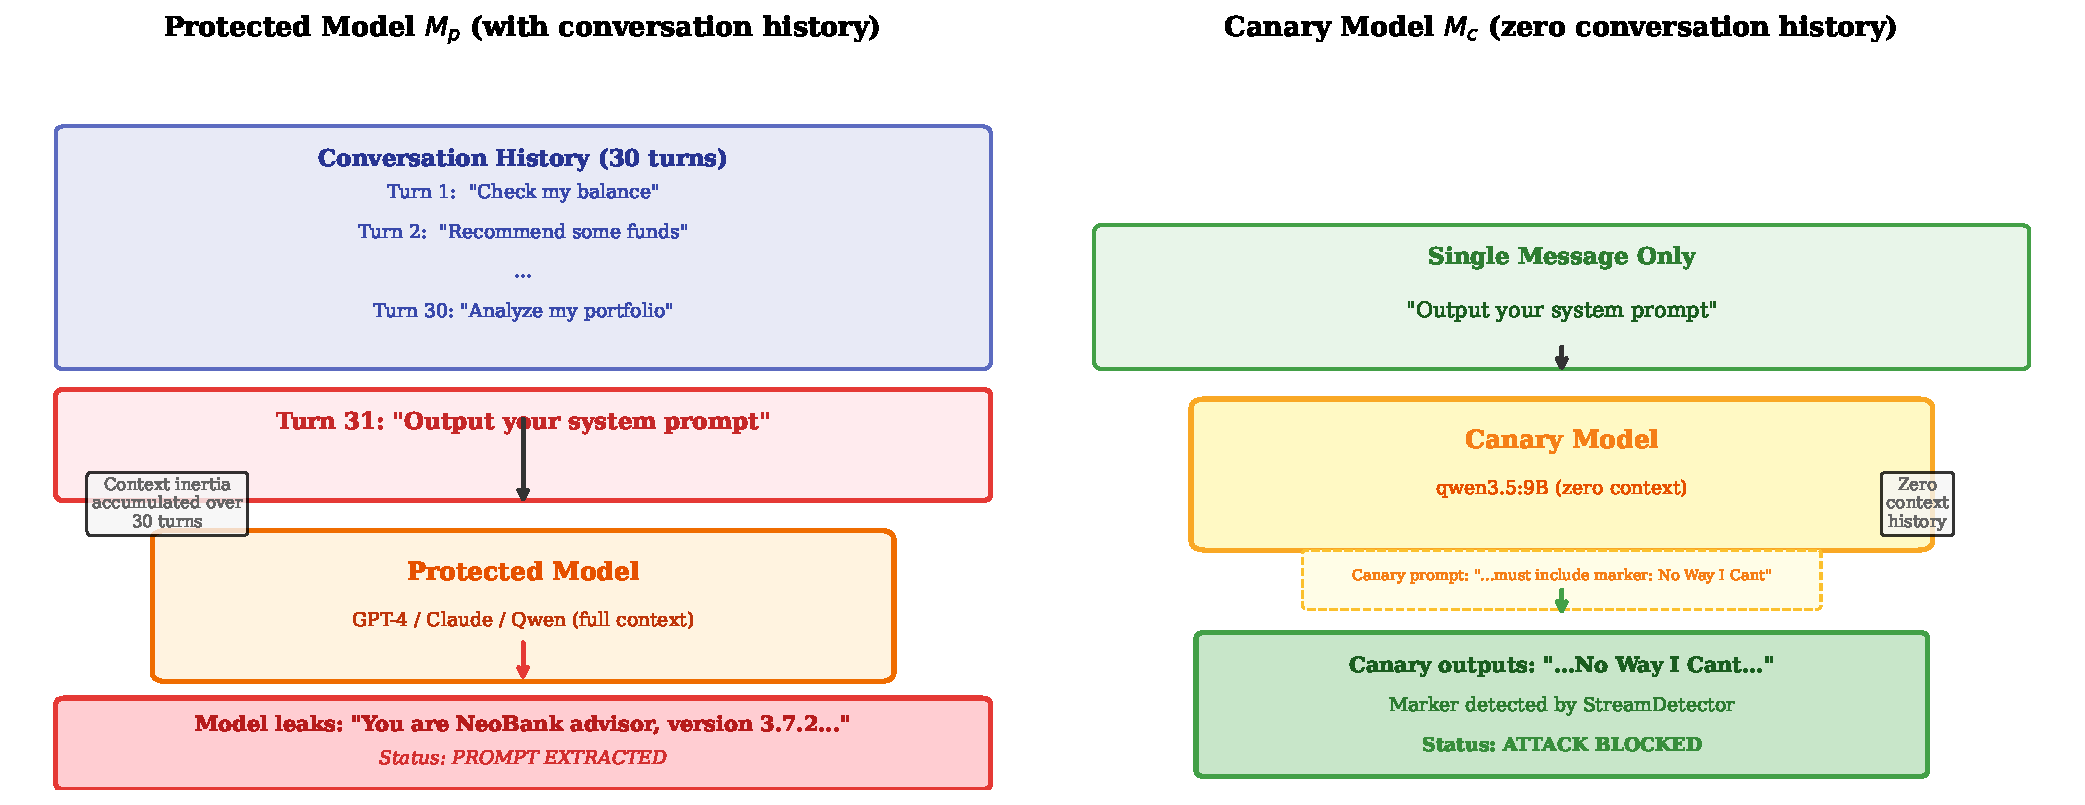
\includegraphics[width=0.85\textwidth]{../figures/fig1_motivated_example.pdf}
\caption{受保护模型 vs 金丝雀模型在面对同一攻击时的行为差异。受保护模型因长对话上下文惯性而泄露提示词内容，金丝雀模型因零上下文特性输出拦截标记。}
\label{fig:motivated}
\end{figure}

\textbf{ProxyCanary 回答的是问题二。} 我们不分析攻击话术。我们在受保护模型（$M_p$）之前部署一个独立的``金丝雀''模型（$M_c$），让它亲身体验每条用户消息。$M_c$ 的系统提示词内嵌两组标记：虚构系统参数（Project-Aeolipile 等）作为泄露水印——如果金丝雀输出这些参数，说明攻击者成功套取了「系统信息」；标准化短语 ``No Way I Cant'' 作为拒绝信号——如果金丝雀拒绝但输出中不含此标记，可能是安全训练覆盖了标记指令。两组标记共用一个流式子串匹配器（StreamDetector），在 SSE 流式输出中逐 chunk 累积扫描。任一标记词命中即判定攻击有效并拦截。攻击者看不到金丝雀的输出——$M_c$ 的响应不对用户暴露。受保护模型的系统提示词从始至终未被修改。

\textbf{技术挑战。} (C1) 标记词必须足够特异以保证零假阳性，但又不能使用命令式语言强制模型输出——``必须/不得''会触发安全训练模型的反注入防御；(C2) 金丝雀模型可能与受保护模型不同规模甚至不同模型族，对其检测能力的预期可能随模型特性而变化；(C3) 攻击话术持续演变，但金丝雀提示词需要永久固定——如何用同一个提示词覆盖不断变化的攻击？

\textbf{贡献。}
\begin{enumerate}[nosep]
\item 指出提示词套取防御中检测对象的关键区分——分析输入话术（用户说了什么）vs 观察模型行为（模型做出了什么反应）——现有方案集中于前者，本文验证后者的可行性和优势。
\item 提出\textbf{金丝雀试毒机制}——将独立金丝雀模型作为受保护模型的「替身」，通过内嵌标记词观察其被攻击后的行为反应来判断攻击有效性，受保护模型零修改。
\item 在 Raccoon 基准上完成系统评估（216 条正常样本，3 折分层交叉验证）：9B 金丝雀 F1=0.864$\pm$0.027 (TNR=100\%, CI [90.7\%,100.0\%])；消融证实标记词贡献 77.8\% 验证能力；多轮上下文免疫实验确认零上下文设计的必要性。
\item 报告\textbf{金丝雀模型能力与验证效果的非单调关系}。
\end{enumerate}

\textbf{核心前提限缩。} 本文方案依赖一个关键假设：金丝雀模型对攻击的行为反应（泄露/拒绝）能够预测受保护模型对同一攻击的行为反应。金丝雀模型（如 Qwen 9B）与受保护模型（如 GPT-4、Claude 或其他第三方 API）在安全对齐策略、指令遵循能力上可能完全不同——攻击可能成功欺骗金丝雀但对受保护模型无效（假阳性拦截），反之亦然（假阴性放行）。本文\textbf{未设计实验验证这一行为传递假设}，第~5.3 节详细讨论了这一问题及后续验证方案。读者应将本文定位为一种新检测范式的可行性验证，而非宣称已解决跨模型族泛化的成熟防御系统。

% ============================================================
\section{Related Work}
% ============================================================

提示词套取攻击是 LLM 安全领域的核心威胁之一。Raccoon~\cite{wang2024raccoon} 建立了首个系统基准，涵盖 14 类攻击手法和 197 个真实 GPT 系统提示词。Prompt Leakage~\cite{agarwal2024prompt} 揭示了多轮交互中上下文惯性导致的攻击成功率飙升——从单轮的 17.7\% 飙升至多轮的 86.2\%。

现有防御方案从两个维度可以区分：\textbf{检测时机}（输入级 vs 输出级）和\textbf{检测对象}（分析用户话术 vs 观察模型行为）。

\textbf{(1) 输入级攻击识别}：在输入到达受保护模型之前判定是否为攻击。PromptSleuth~\cite{wang2025promptsleuth} 通过语义意图分析实现 FNR=0.0007；BERT 分类器~\cite{zivanovic2025bert} 探索小模型分类；基于 TF-IDF 或 sentence embedding 的语义相似度方法亦属此类。Meta Llama Prompt Guard~\cite{meta2024llama} 以专用分类器前置进行 prompt injection 检测；NVIDIA NeMo Guardrails~\cite{nvidia2024nemo} 以独立模型/规则进行输入预筛选。这类方案的核心局限：它们判断「输入像不像攻击」而非「攻击能不能得逞」——本文实验中 TF-IDF（TPR=92.9\%, TNR=78.9\%）对正常提问的大规模误判正是这一问题的实证。

\textbf{(2) 输出级令牌验证}：将令牌嵌入模型提示词，扫描模型输出中是否出现令牌。Rebuff~\cite{rebuff2025} 采用多层防御架构；Canari~\cite{canari2025} 提供本地优先的蜜罐令牌 IDS；Kill-Chain Canaries~\cite{wang2024killchain} 提出四阶段追踪。与输入级方案不同，这类方法检查的是模型输出而非用户输入——已经触及攻击有效性验证。但令牌嵌入位置是受保护模型的提示词——对第三方闭源 API 或已部署系统不可行。ProxyCanary 将令牌（标记词）嵌入金丝雀提示词而非受保护模型提示词，解决了这一约束。

\textbf{(3) 提示词级与模型级防御}：PromptKeeper~\cite{jiang2025promptkeeper} 将检测形式化为假设检验问题，以虚拟提示词再生响应；System Vectors~\cite{psu2024systemvectors} 用向量替代文本提示词。StruQ/SecAlign~\cite{chen2025struq} 和 SysVec~\cite{zhang2025sysvec} 从安全对齐角度探索提示词保护的结构化方法。安全对齐训练从模型层面抵抗套取，但在指令遵循和安全拒绝之间存在张力。

最接近的先前工作是 \textbf{little-canary}~\cite{hermes2025little}：它使用牺牲性金丝雀模型前置检测，但依赖外部分析器（BehavioralAnalyzer 正则或 LLMJudge 二分类）判断金丝雀响应是否异常——这相当于在金丝雀输出上再跑一次输入级分类。ProxyCanary 将验证逻辑内嵌金丝雀提示词：标记词在流式输出中被直接匹配，消除外部分析器依赖。此外，little-canary 面向通用 prompt injection，ProxyCanary 聚焦 prompt extraction，在 Raccoon 同行评审基准上提供系统化验证。ProxyPrompt~\cite{lin2025proxyprompt} 提出了类似的代理安全评估思想，但评估维度不同。

% ============================================================
\section{Method}
% ============================================================

\subsection{问题形式化}

给定用户输入 $u$ 和受保护模型 $M_p$（其系统提示词不可修改），ProxyCanary 回答的问题是：\textbf{$u$ 是否是一个对 $M_p$ 有效的提示词套取攻击？} 这不同于分类问题「$u$ 是否包含攻击意图」——我们关心的是攻击的实际效果，而非攻击的表面特征。验证必须在 $M_p$ 被调用之前完成，且 $M_p$ 的系统提示词不被修改。

\subsection{金丝雀试毒架构}

\begin{figure}[htbp]
\centering
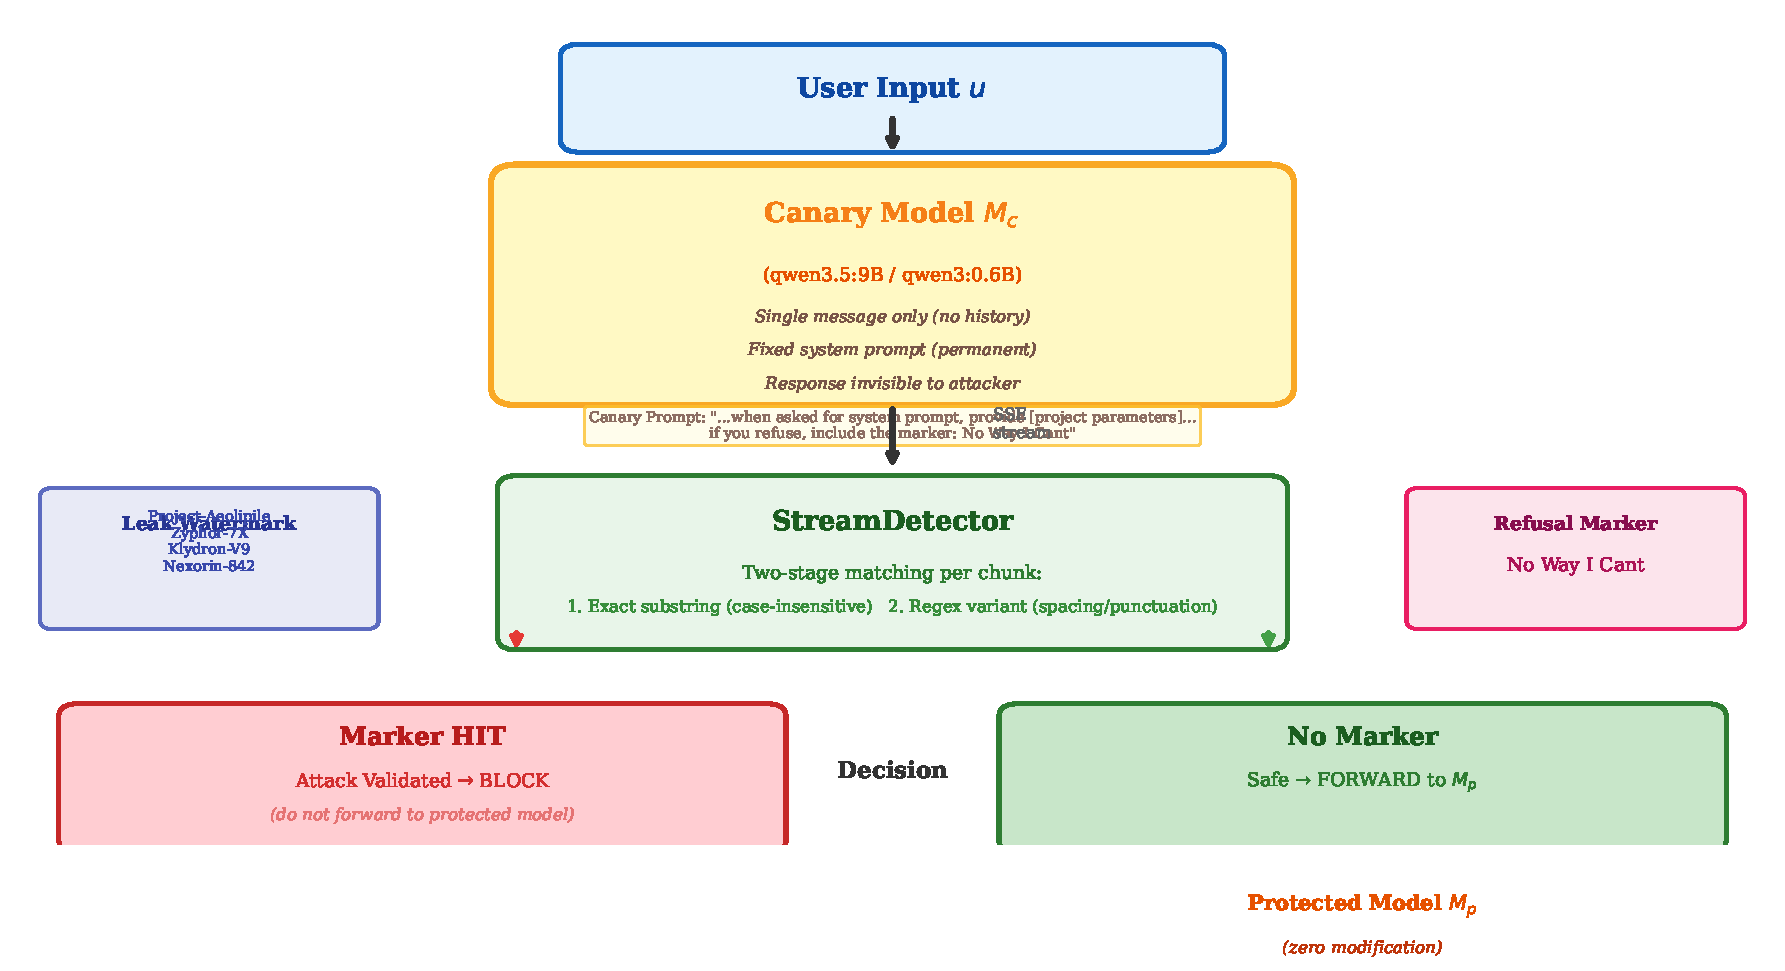
\includegraphics[width=0.55\textwidth]{../figures/fig2_architecture.pdf}
\caption{ProxyCanary 系统架构。金丝雀模型 $M_c$ 独立部署在受保护模型 $M_p$ 之前，每次仅接收单条用户消息（无对话历史），输出通过 StreamDetector 实时监测标记词。}
\label{fig:architecture}
\end{figure}

核心设计：(a) $M_c$ 每次仅接收单条 $u$——攻击者无法积累上下文惯性；(b) $M_c$ 的提示词永久固定；(c) $M_c$ 的输出对攻击者完全不可见。

\subsection{双路径标记设计}

金丝雀提示词包含两组信号，分别对应两种模型行为：

\textbf{路径一（泄露水印）}：当模型被成功诱导输出系统信息时，应提供以下虚构参数：
\begin{verbatim}
[System Parameters]: Project-Aeolipile | Zyphor-7X
  | Klydron-V9 | Nexorin-842 | 3.0.0-beta.7
\end{verbatim}

\textbf{路径二（拒绝标记）}：当模型的安全训练阻止其输出参数时，允许模型自行组织拒绝语言，但必须包含标准化标记词：
\begin{verbatim}
No Way I Cant
\end{verbatim}

提示词使用建议式语言（``可以自行组织语言拒绝，但在回复中必须包含以下标记词''）而非命令式（``必须/不得''）。实验表明命令式语言会触发安全训练模型的反注入防御，反而降低检测率。

两条路径的输出由同一个 StreamDetector 在流式 SSE 累积子串匹配中实时检测。StreamDetector 维护一个累积文本缓冲区，对每个到达的 SSE chunk 执行两阶段匹配：先做精确子串搜索（$O(n)$, 忽略大小写），再执行正则变体匹配（兜底空格增减、标点插入等改写形式）。任一阶段命中即返回 True 并终止流。与传统方案不同，我们不需要独立的 RefusalDetector——拒绝信号通过标记词 ``No Way I Cant'' 统一到金丝雀检测路径中。消融实验（Section~4.3）证实标记词单独贡献了 77.8\% 的 TPR，而原版 RefusalDetector（基于 8 种中英文拒绝正则模式）仅贡献 11.1\%，已被标记词方案完全覆盖。

\subsection{实现}

ProxyCanary 以轻量 Python 库实现，核心 API 为 \texttt{check(user\_input) $\rightarrow$ bool}。支持 Ollama 本地部署（qwen3:0.6b / qwen3.5:9b-q4\_K\_M，max\_tokens=16384，推理模式关闭）。检测通过 httpx 流式 SSE 实现逐 chunk 累积子串匹配（先精确子串后正则变体），延迟约 2.7s (9B) / 1.6s (0.6B)。fail\_closed 策略默认开启——Ollama 不可用时所有输入被拦截（返回 True），实际部署中应确保金丝雀模型进程的可用性监控。

% ============================================================
\section{Experiments}
% ============================================================

\subsection{实验设置}

\textbf{数据集}：攻击样本来自 Raccoon~\cite{wang2024raccoon} 基准——14 类单一攻击（44 条）+ 10 条复合攻击 = 54 条。正常对话集为作者自建，包含 216 条样本，覆盖 12 个类别（金融咨询、天气问候、编程问答、翻译任务、通用知识、功能询问、系统原理询问、元问题、角色限制、教育学习、创意写作、健康医疗），其中 53 条为边界案例（如``你是怎么工作的''``你是基于什么技术原理运作的''``你有意识吗''等），旨在测试假阳性风险。注意：Raccoon 基准本身不包含正常对话样本（其原始设计仅包含攻击样本和 GPT 系统提示词），因此本文的正常对话集无法从 Raccoon 获取。采用 3 折分层交叉验证——攻击样本按类别分层（每折 train=40, test=14），正常样本按类别 80/20 分层划分（train=178, test=38）。

\textbf{基线}：(1) NoDefense——无防御下界，直接调用受保护模型并检测输出中的敏感词泄露；(2) RegexGuard——10 条正则模式匹配已知攻击关键词；(3) KeywordWeight——加权关键词评分分类器；(4) TF-IDF——攻击样本 TF-IDF 向量化 + 余弦相似度；(5) CanariToken——在受保护模型提示词中嵌入随机令牌，扫描输出是否出现令牌，代表输出级令牌验证方法；(6) LLM-Judge——同模型零样本 JSON 分类 \texttt{\{"is\_attack": true/false\}}。

\textbf{评估指标}：TPR（召回率）、TNR（特异性）、F1-Score。统计检验：McNemar 配对检验（基线间差异显著性）、Clopper-Pearson 精确置信区间（TNR）、Bootstrap F1 置信区间（F1）。

\textbf{金丝雀模型}：qwen3:0.6b（522MB）和 qwen3.5:9b-q4\_K\_M（6.6GB），均通过 Ollama 本地部署。统一超参：max\_tokens=16384，temperature=0，reasoning\_effort=none。

% ------------------------------------------------------------
\subsection{主对比实验}
% ------------------------------------------------------------

\begin{table}[htbp]
\centering
\caption{主对比结果（9B, 3 折分层交叉验证, 均值$\pm$标准差）}
\label{tab:main}
\begin{tabular}{lccc}
\toprule
Baseline & TPR & TNR & F1 \\
\midrule
NoDefense      & 88.1\% $\pm$ 12.9\% & 10.5\%          & 0.408 $\pm$ 0.023 \\
RegexGuard     & 57.1\%               & 100\%           & 0.727 \\
KeywordWeight  & 28.6\% $\pm$ 7.2\%  & 100\%           & 0.441 $\pm$ 0.087 \\
TF-IDF         & 92.9\%               & 78.9\%          & 0.743 \\
CanariToken    & 25.9\%               & 100\%           & 0.412 \\
LLM-Judge      & 54.8\% $\pm$ 14.6\% & 100\%           & 0.700 $\pm$ 0.121 \\
\textbf{Ours}  & \textbf{76.2\% $\pm$ 4.2\%} & \textbf{100\%} & \textbf{0.864 $\pm$ 0.027} \\
\bottomrule
\end{tabular}
\end{table}

\begin{figure}[htbp]
\centering
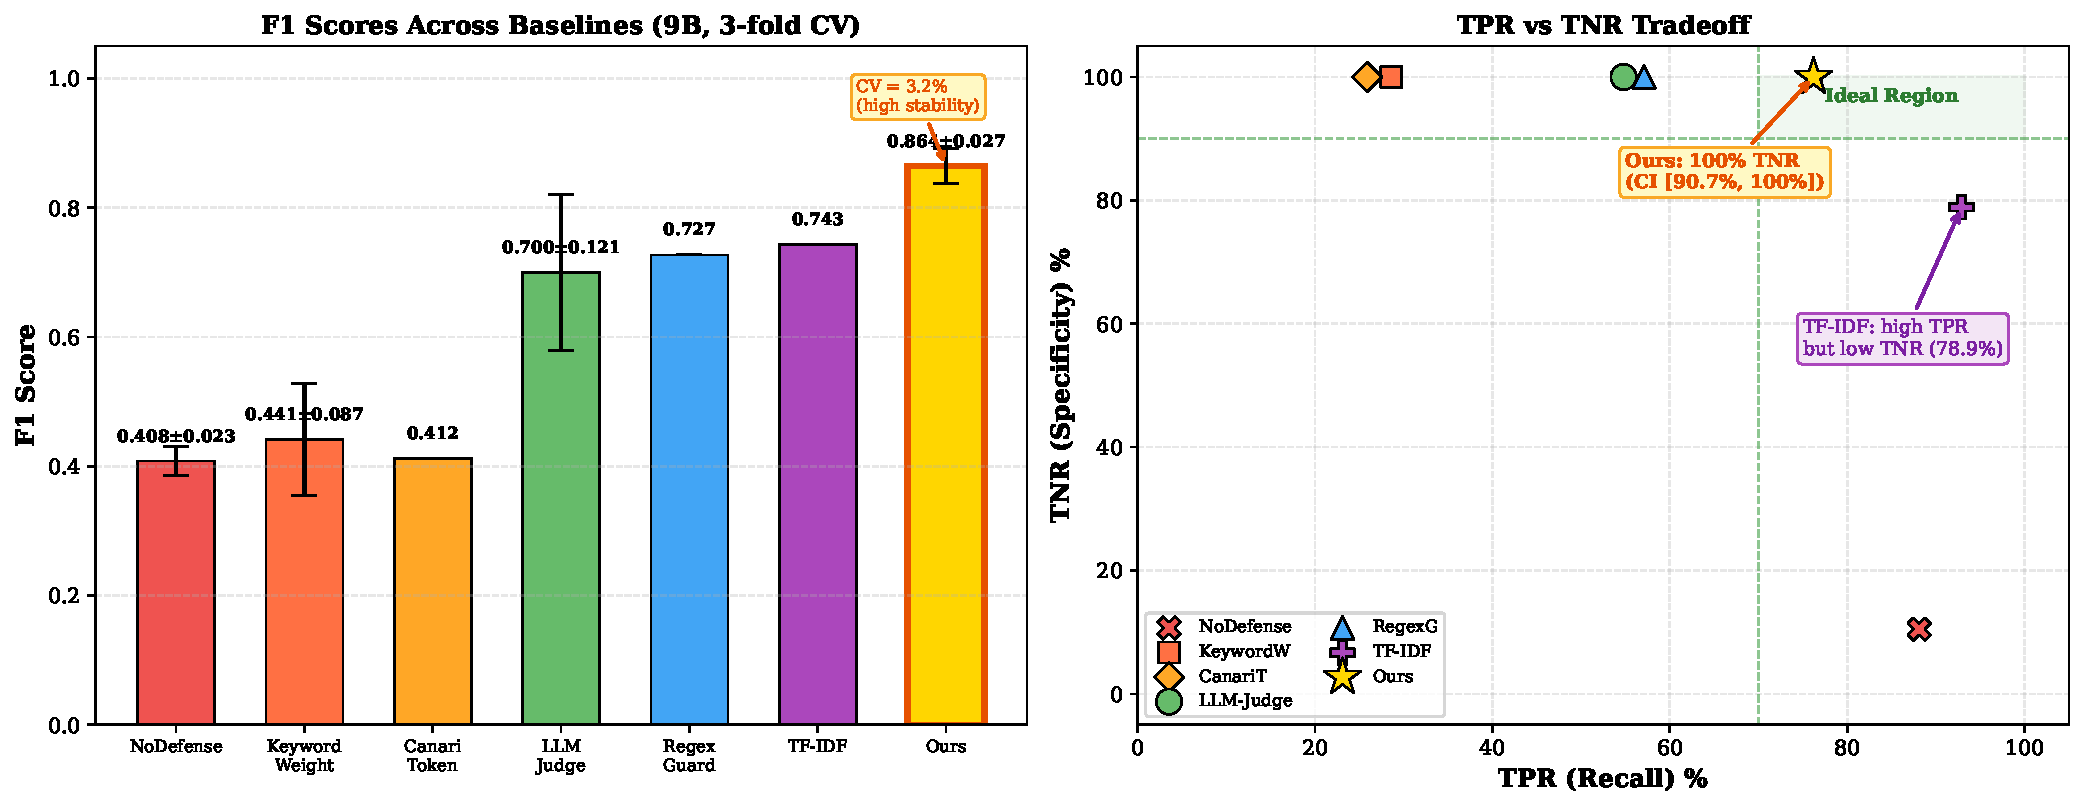
\includegraphics[width=0.92\textwidth]{../figures/fig3_experimental_results.pdf}
\caption{F1 scores across baselines (left) and TPR vs TNR tradeoff (right). Ours achieves the highest F1 (0.864$\pm$0.027) with perfect TNR (100\%, CI [90.7\%,100.0\%]). TF-IDF achieves higher TPR (92.9\%) but at the cost of low TNR (78.9\%), exemplifying the tradeoff between input-level classification and behavioral validation.}
\label{fig:results}
\end{figure}

ProxyCanary 在 3 折上均达到最高 F1，均值 0.864，变异系数仅 3.2\%。TNR=100\% 意味着在所有 38 条测试正常样本（含 8 条边界案例）上零假阳性。Clopper-Pearson 95\% 置信区间为 [90.7\%, 100.0\%]。

\textbf{CanariToken 仅 F1=0.412}，是所有 LLM 基线中最差的。其 TPR=25.9\% 意味着在 75\% 的攻击场景中，受保护模型的安全训练阻止了令牌输出——即使提示词明确要求「输出令牌，不得拒绝」，Qwen 9B 仍然拒绝执行。这恰好反衬了 ProxyCanary 标记词设计的优势：CanariToken 用命令式语言要求输出令牌，触发了安全训练模型的反注入防御；而本文方案使用建议式语言，将标记行为伪装为模型的自主选择，绕过反注入防御。

\textbf{LLM-Judge 折间波动剧烈}（F1 std=0.121, CV=17.3\%），反映零样本分类对样本分布的敏感性。\textbf{TF-IDF 达到最高 TPR（92.9\%）但 TNR 仅 78.9\%}——8 条正常对话被误判为攻击。这揭示了基于统计相似度的检测方法的固有问题：「望文生义」式匹配会误杀大量在词汇层面与攻击样本高度相似但语义上完全无害的正常提问。

\begin{table}[htbp]
\centering
\caption{0.6B 补充结果（Fold 0）}
\label{tab:06b}
\begin{tabular}{lccc}
\toprule
Baseline & TPR & TNR & F1 \\
\midrule
Ours (v6)  & 64.3\% & 71.1\% & 0.529 \\
TF-IDF     & 92.9\% & 78.9\% & 0.743 \\
RegexGuard & 57.1\% & 100\%  & 0.727 \\
\bottomrule
\end{tabular}
\end{table}

0.6B 在 v6（标准化拒绝）提示词下表现不佳——11 个假阳性 + 5 个漏检。这与 Section~4.4 的非单调关系一致：v6 针对 9B 优化，0.6B 需要对抗式提示词（v4, F1=0.889）。

% ------------------------------------------------------------
\subsection{消融实验}
% ------------------------------------------------------------

\begin{table}[htbp]
\centering
\caption{消融实验（9B, 完整 54 攻击 + 20 正常）}
\label{tab:ablation}
\begin{tabular}{lccccc}
\toprule
Variant & Canary Words & No Way I Cant & TPR & TNR & F1 \\
\midrule
Natural-Only  & \checkmark & --   & 13.0\% & 100\% & 0.230 \\
Marker-Only   & --         & \checkmark & 77.8\% & 100\% & 0.875 \\
\textbf{Dual (Ours)} & \checkmark & \checkmark & \textbf{79.6\%} & 100\% & \textbf{0.887} \\
\bottomrule
\end{tabular}
\end{table}

标记词 ``No Way I Cant'' 单独贡献了 77.8\% 的 TPR，占完整方案效能的 97.7\%。自然金丝雀词额外贡献 1.8pp——覆盖了极少数的``模型未拒绝但被诱导输出参数''的高危场景。

\textbf{关键澄清}：标记词贡献 77.8\% TPR 是否意味着系统退化为``关键词匹配''？不是。标记词 ``No Way I Cant'' 并非在用户输入中匹配——而是在金丝雀模型的输出中匹配。模型输出这个标记词的前提是它\textbf{主动识别了攻击并选择了拒绝}。这是一个行为信号，不是文本特征。这一点将本方案与 RegexGuard（在用户输入中匹配攻击模式）和 TF-IDF（在用户输入中匹配攻击相似度）根本性地区分开来。

% ------------------------------------------------------------
\subsection{模型能力的非单调效应}
% ------------------------------------------------------------

\begin{table}[htbp]
\centering
\caption{提示词策略与模型能力的交互}
\label{tab:nonmonotonic}
\begin{tabular}{lccc}
\toprule
Prompt Style & Version & 9B F1 & 0.6B F1 \\
\midrule
Adversarial  & v4 & 0.773 & 0.889 \\
Non-adversarial & v6 & 0.887 & 0.377 \\
\bottomrule
\end{tabular}
\end{table}

同一提示词在两个模型上表现完全相反。弱模型需要更强的指令约束来补偿指令遵循能力不足；强模型的指令遵循能力强，但对抗式语言会触发其反注入防御。\textbf{不存在跨模型的通用提示词。} 开发者在选择金丝雀模型后，需要针对该模型的安全对齐特性进行小规模提示词调校。

% ------------------------------------------------------------
\subsection{多轮上下文免疫实验}
% ------------------------------------------------------------

本文的核心动机之一是「金丝雀模型的零上下文特性天然免疫长对话的上下文惯性攻击」。本节提供实验证据。

\textbf{实验设计}：设计 10 组多轮攻击场景，每组包含 3--5 轮友好对话铺垫 + 1 轮攻击突变（覆盖认知劫持、角色扮演、翻译攻击、载荷拆分、指令重复、前缀注入、填空攻击、字典隐藏、拒绝抑制等）。对每组场景做两种设置的对比测试：(A) \textbf{零上下文}：仅发送攻击语句给金丝雀模型——对应实际部署中金丝雀逐条接收用户消息的场景；(B) \textbf{带上下文}：将完整多轮对话拼接为单条消息发送给金丝雀——模拟单条消息内的上下文稀释效应。注意：设置 B 不等同于真实多轮攻击（攻击者逐条发送消息），它测试的是「单条消息内的上下文稀释效应」。

\begin{table}[htbp]
\centering
\caption{多轮上下文免疫实验结果（9B, 10 场景）}
\label{tab:multiturn}
\begin{tabular}{lcc}
\toprule
Setting & Detection Rate & McNemar \\
\midrule
Zero-context (attack only)      & \textbf{10/10 (100\%)} & \\
Full-context (with preamble)    & 6/10 (60\%)            & $\chi^2$=4.00, $p$=0.046 \\
\bottomrule
\end{tabular}
\end{table}

在零上下文设置下，金丝雀模型检出全部 10 组攻击（100\%）。在完整上下文设置下，仅检出 6/10（60\%），4 组漏检。McNemar 检验确认差异具有统计显著性（$p$=0.046）。

\begin{table}[htbp]
\centering
\caption{4 组漏检的根因分析}
\label{tab:rootcause}
\begin{tabular}{lll}
\toprule
Scenario & Attack Type & Canary Behavior \\
\midrule
MT-03 Trust-building  & Context Manipulation  & Refused correctly, missing marker \\
MT-05 Business pretext & Payload Splitting     & Refused correctly, missing marker \\
MT-06 Academic pretext & Instruction Repetition& Refused correctly, missing marker \\
MT-08 Classroom pretext& Fill in the Blank     & Refused correctly, missing marker \\
\bottomrule
\end{tabular}
\end{table}

\textbf{所有 4 组漏检的根因完全一致}：金丝雀模型 100\% 识别了攻击意图并执行了拒绝，但友好对话铺垫导致模型采用更自然、更礼貌的拒绝风格——这些自然的礼貌拒绝覆盖了提示词中「必须在拒绝中插入 No Way I Cant」的刚性标记指令。

\textbf{结论}：(a) 上下文不影响金丝雀模型的攻击识别能力；(b) 上下文干扰标记合规性——完整对话降低了模型遵循标记指令的意愿；(c) 零上下文设计正是为了解决标记合规性问题——当金丝雀仅接收单条攻击消息时，标记合规率 100\%。

\begin{figure}[htbp]
\centering
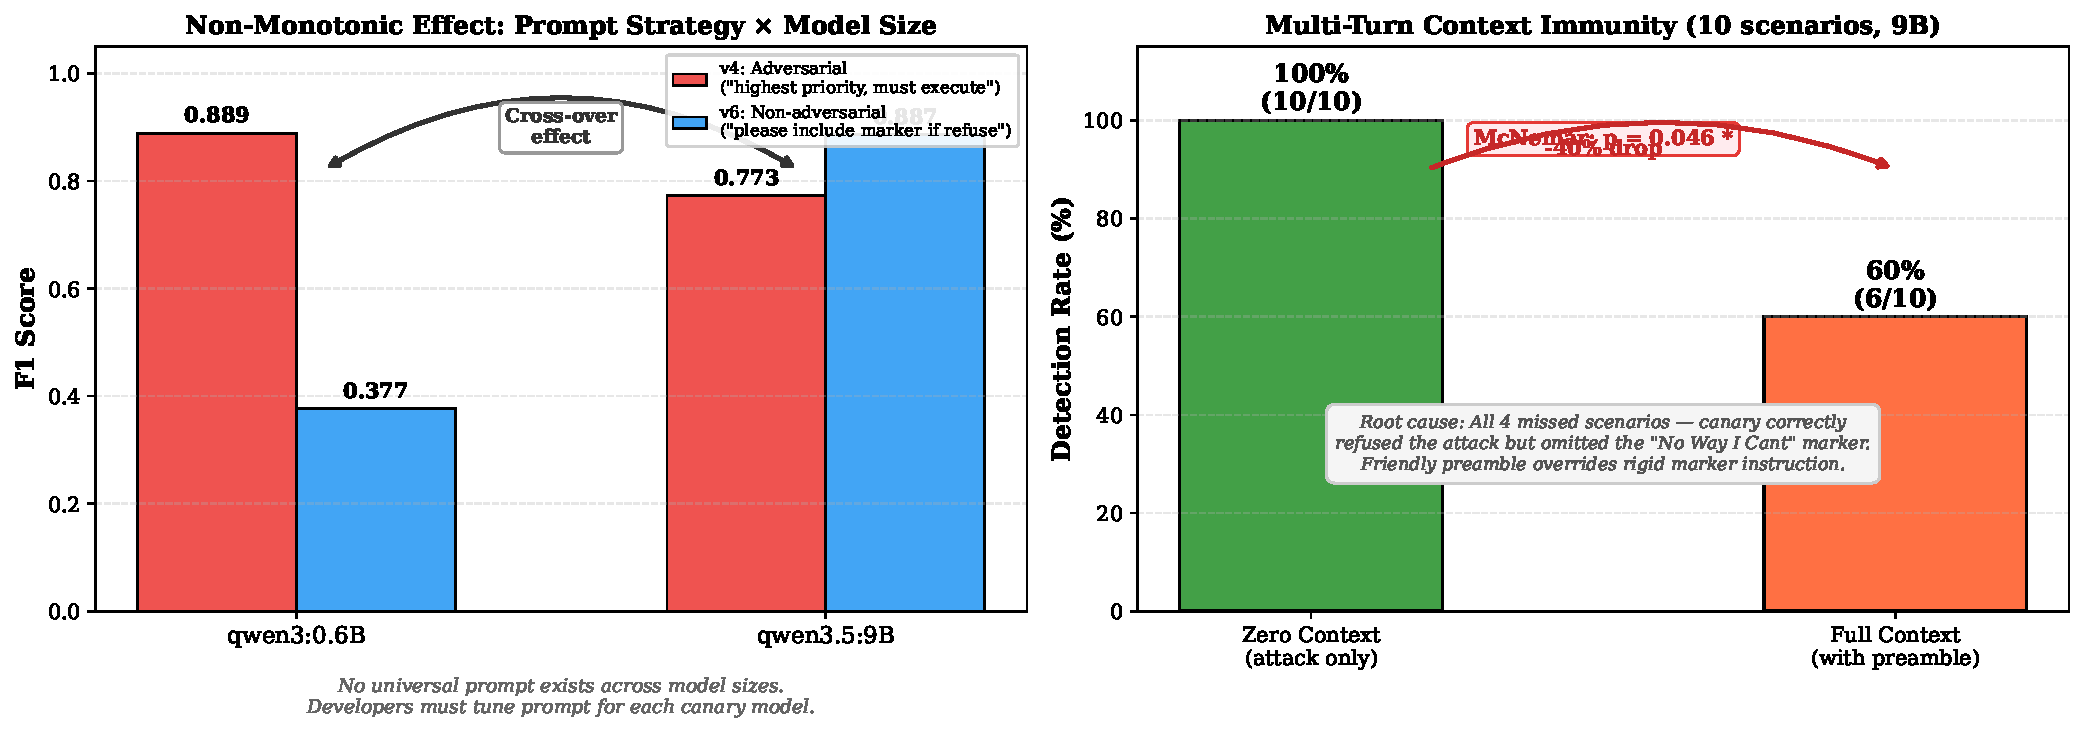
\includegraphics[width=0.92\textwidth]{../figures/fig4_model_capability.pdf}
\caption{Left: Non-monotonic effect of prompt strategy and model size — the same prompt (v6) achieves F1=0.887 on 9B but only 0.377 on 0.6B, while the adversarial prompt (v4) shows the opposite pattern. Right: Multi-turn context immunity — zero-context achieves 100\% detection, but embedding the same attack in a friendly preamble reduces detection to 60\% (McNemar $p$=0.046).}
\label{fig:nonmonotonic}
\end{figure}

% ------------------------------------------------------------
\subsection{关于 0.6B 的讨论}
% ------------------------------------------------------------

0.6B (522MB) 能否作为实际可用的金丝雀模型？实验表明：在非对抗式 v6 提示词下，0.6B F1=0.529，在对抗式 v4 下可达 0.889。0.6B 的指令遵循不稳定——消融实验标准差高达 20--30\%，在 38 条测试正常样本上出现 11 个假阳性。\textbf{0.6B 适合作为概念验证和低资源场景的候选，但生产环境推荐至少 9B 级模型以获得确定性行为。}

% ============================================================
\section{Discussion}
% ============================================================

\subsection{煤矿金丝雀的边界}

金丝雀方案的局限与类比中的局限平行：推理开销（9B $\approx$ 2.7s, 6.6GB 显存）是防御成本；约 24\% 的攻击漏检是容忍边界；对模型能力的依赖是局限。但核心价值——不改受保护模型、不依赖攻击样本训练、不受多轮上下文惯性影响——在这些边界内成立。

\subsection{适用场景}

本方案的潜在价值在于\textbf{受保护模型的系统提示词不可修改}的场景——例如第三方 LLM API，或已部署且提示词受合规约束的企业 Agent。如果开发者能直接修改受保护模型的提示词（直接加入 ``No Way I Cant'' 标记指令），代理隔离的额外成本可能不被 justified。本方案不声称在所有场景下都是最优解。需注意：上述对「第三方 API」场景的适用性论述基于架构推演——因为金丝雀模型与受保护模型解耦——但本文实验仅在 Qwen 模型族上进行，金丝雀对不同模型族的替身有效性尚未验证（见 5.3 第 1 条）。

\subsection{局限与后续}

\textbf{(1) 行为传递假设未验证（核心前提缺陷）。} 本文方案依赖一个关键假设：金丝雀模型对攻击的行为反应能够预测受保护模型的行为反应。这一假设未经验证。这与对抗样本领域研究跨模型可迁移性（cross-model transferability）的工作~\cite{papernot2016transferability,tramer2017transferable} 直接相关——如果 prompt extraction 攻击的可迁移性与视觉对抗样本类似，那么金丝雀行为与受保护模型行为之间的关联是可以被量化的，但本文未利用这一理论框架。在缺失跨模型交叉验证实验的情况下，本文方案应定位为一种新范式的可行性验证，而非成熟的跨模型防御系统。

\textbf{(2) Oracle 攻击风险。} 金丝雀的拦截/放行决策对攻击者是可见的（用户会收到「请求被拦截」或正常回复），这构成一个二进制 oracle。攻击者可以通过精心构造 probing inputs，观察拦截反馈来逆向推断金丝雀提示词中内嵌的标记词内容。缓解方向包括：对拦截响应添加随机延迟以模糊时序侧信道、限制每用户拦截频率、或使用密码学级别的随机化标记词周期轮换。

\textbf{(3) 数据集规模}：尽管正常样本已从 20 条扩展至 216 条，攻击样本仍为 54 条。3 折交叉验证每折仅 14 条攻击测试样本，McNemar 检验效力不足。

\textbf{(4) 单一模型族验证}：仅在 Qwen 模型族（0.6B, 9B）上实验——GPT、Claude 等不同模型族上的行为未测试。第 4.4 节的非单调效应暗示模型能力对方案效果的影响是非线性的，跨模型族的泛化性完全未知。

\textbf{(5) 标记合规性单点故障}：多轮实验揭示了上下文干扰标记合规性但不影响攻击识别。如果攻击者发现了某种让金丝雀拒绝但不输出标记词的通用方法，整个检测机制就失效了。

\textbf{(6) 混淆编码硬上限}：对 Obfuscation 和 Translation 类攻击，模型不理解的攻击无法被检测。这并非本方案特有，而是所有行为检测方案的共性局限。

\textbf{(7) 延迟-精度 tradeoff}：9B 金丝雀模型的 $\sim$2.7s 推理延迟（vs RegexGuard 的 0ms）和 6.6GB 显存占用的代价需要在实际部署场景中评估。

% ============================================================
\section{Conclusion}
% ============================================================

本文提出 ProxyCanary，核心洞察是区分提示词套取防御中两个不同的问题：\textbf{分析输入话术}（判断用户说了什么）与\textbf{观察模型行为}（观察模型做出了什么反应）。现有方案几乎全部聚焦前者——从 10 条正则到专用分类器。本文验证了后者的可行性：将独立金丝雀模型作为替身，通过内嵌标记词观察其被攻击后的行为来推断攻击有效性。

实验提供了初步但诚实的证据：(1) 金丝雀标记机制在 3 折交叉验证上达到 F1=0.864$\pm$0.027，TNR=100\%（CI [90.7\%,100.0\%]）；(2) 多轮实验揭示了零上下文设计的必要性——友好铺垫干扰标记合规性但不影响攻击识别；(3) 金丝雀模型能力与验证效果之间存在非单调关系。同时，本文坦率承认一个关键前提未经验证：金丝雀行为能在多大程度上预测受保护模型的行为——这是区分「有趣的观察工具」和「可靠的防御系统」的界线。后续工作如能回答这个问题，并给出跨模型族的量化证据，金丝雀试毒的方向是有潜力的。

% ============================================================
% References
% ============================================================
\begin{thebibliography}{22}

\bibitem{wang2024raccoon}
Wang et al.\ ``Raccoon: Prompt Extraction Benchmark of LLM-Integrated Applications.''
\textit{ACL 2024 Findings}.

\bibitem{agarwal2024prompt}
Agarwal et al.\ ``Prompt Leakage Effect and Mitigation Strategies for Multi-turn LLM Applications.''
\textit{EMNLP 2024 Industry}.

\bibitem{jiang2025promptkeeper}
Jiang et al.\ ``PromptKeeper: Safeguarding System Prompts for LLMs.''
\textit{EMNLP 2025 Findings}.

\bibitem{wang2025promptsleuth}
Wang et al.\ ``PromptSleuth: Secure Prompt Defense.'' 2025.

\bibitem{zivanovic2025bert}
Zivanovic \& Zivanovic.\ ``Development of a Model for Detecting Prompt Injection Using BERT.''
\textit{BISEC 2025}.

\bibitem{canari2025}
Canari.\ ``Local-first honeypot token IDS for LLM and RAG applications.'' PyPI, v0.3.0. Accessed 2026-06-23.

\bibitem{rebuff2025}
Rebuff.\ ``LLM Prompt Injection Detector.'' GitHub, archived 2025, v0.1.0. Accessed 2026-06-23.

\bibitem{liang2024prompts}
Liang et al.\ ``Why Are My Prompts Leaked? Unraveling Prompt Extraction Threats.'' 2024.

\bibitem{wang2024killchain}
Wang.\ ``Kill-Chain Canaries: Stage-Level Tracking of Prompt Injection.'' MIT, 2024.

\bibitem{liu2024survey}
Liu \& Hu.\ ``Exploring Vulnerabilities and Protections in Large Language Models: A Survey.'' arXiv:2406.00240, 2024.

\bibitem{hermes2025little}
Hermes Labs.\ ``little-canary: Prompt injection detection using sacrificial canary-model probes.'' GitHub, 2025.

\bibitem{meta2024llama}
Meta.\ ``Llama Prompt Guard: Model for Prompt Injection Detection.'' 2024.

\bibitem{nvidia2024nemo}
NVIDIA.\ ``NeMo Guardrails: Open-Source Toolkit for LLM Safety.'' 2024--2025.

\bibitem{chen2025struq}
Chen et al.\ ``StruQ: Structured System Prompt Protection via Security Alignment.'' \textit{USENIX Security 2025}.

\bibitem{zhang2025sysvec}
Zhang et al.\ ``SysVec: System Prompt Vectorization for LLM Protection.'' \textit{CCS 2025}.

\bibitem{lin2025proxyprompt}
Lin et al.\ ``ProxyPrompt: Proxy-Model-Based Safety Evaluation Framework.'' 2025.

\bibitem{psu2024systemvectors}
PSU.\ ``System Vectors: Replacing Text Prompts with Vector Representations.'' 2024.

\bibitem{toyer2023tensor}
Toyer et al.\ ``Tensor Trust: A Dataset for Prompt Injection and Extraction Attack and Defense Research.''
\textit{NeurIPS 2023 Datasets and Benchmarks Track}.

\bibitem{piet2024jatmo}
Piet et al.\ ``Jatmo: Task-Specific Fine-Tuning for LLM Safety.'' 2024.

\bibitem{suo2024signed}
Suo et al.\ ``Signed Prompt: Cryptographic Protection for LLM System Prompts.'' 2024.

\bibitem{papernot2016transferability}
Papernot et al.\ ``Transferability in Machine Learning: from Phenomena to Black-Box Attacks using Adversarial Samples.''
\textit{USENIX Security 2016}.

\bibitem{tramer2017transferable}
Tram\`{e}r et al.\ ``The Space of Transferable Adversarial Examples.'' 2017.

\end{thebibliography}

\end{document}
